\documentclass{standalone}
\usepackage{PhysicalChemistryNote}
\begin{document}
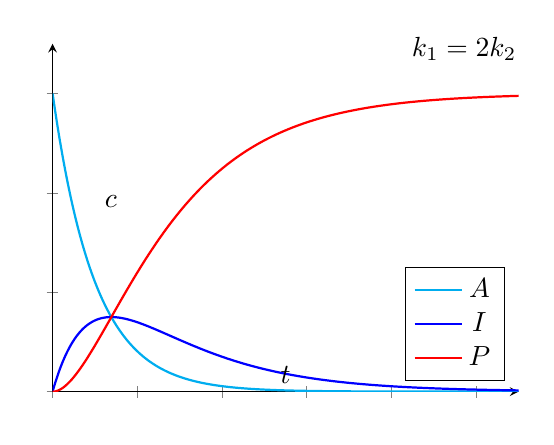
\begin{tikzpicture}
    \begin{axis}[
        title = {$k_1=2k_2$},
        title style={at={(0.75,1)},anchor=north west},
        width = 7.5cm,
        height = 6cm,
        legend pos = south east,
        x label style={at={(axis description cs:0.5,0.1)},anchor=north},
        y label style={at={(axis description cs:0.125,0.5)},rotate=270,anchor=south},
        xlabel = {$t$},
        ylabel = {$c$},
        axis lines = left,
        ymax = 3.5,
        domain = 0:5.5,
        samples = 400,
        xticklabels={},
        yticklabels={}
    ]
    \addplot [thick, cyan] {3*e^(-2*x)};
    \addplot [thick, blue] {3*(e^(-x)-e^(-2*x))};
    \addplot [thick, red] {3*(1-(2*e^(-x)-e^(-2*x)))};
    \legend {$\con{A}$,$\con{I}$,$\con{P}$}
    \end{axis}
\end{tikzpicture}
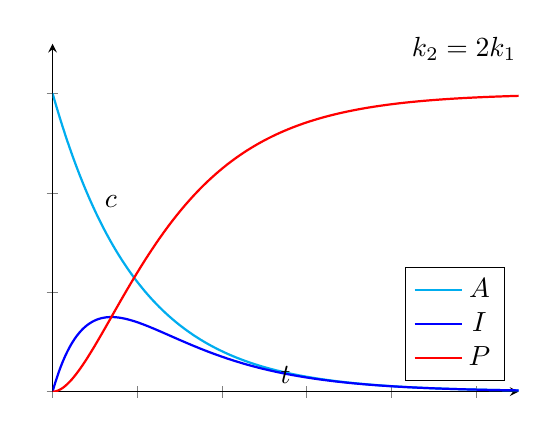
\begin{tikzpicture}
    \begin{axis}[
        title = {$k_2=2k_1$},
        title style={at={(0.75,1)},anchor=north west},
        width = 7.5cm,
        height = 6cm,
        legend pos = south east,
        x label style={at={(axis description cs:0.5,0.1)},anchor=north},
        y label style={at={(axis description cs:0.125,0.5)},rotate=270,anchor=south},
        xlabel = {$t$},
        ylabel = {$c$},
        axis lines = left,
        ymax = 3.5,
        domain = 0:5.5,
        samples = 400,
        xticklabels={},
        yticklabels={}
    ]
    \addplot [thick, cyan] {3*e^(-x)};
    \addplot [thick, blue] {3*(e^(-x)-e^(-2*x))};
    \addplot [thick, red] {3*(1-(2*e^(-x)-e^(-2*x)))};
    \legend {$\con{A}$,$\con{I}$,$\con{P}$}
    \end{axis}
\end{tikzpicture}
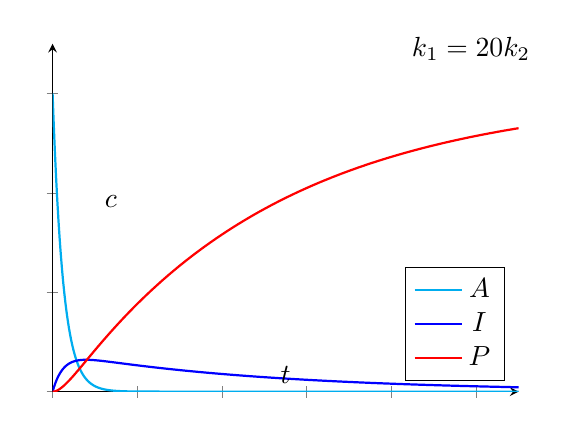
\begin{tikzpicture}
    \begin{axis}[
        title = {$k_1=20k_2$},
        title style={at={(0.75,1)},anchor=north west},
        width = 7.5cm,
        height = 6cm,
        legend pos = south east,
        x label style={at={(axis description cs:0.5,0.1)},anchor=north},
        y label style={at={(axis description cs:0.125,0.5)},rotate=270,anchor=south},
        xlabel = {$t$},
        ylabel = {$c$},
        axis lines = left,
        ymax = 3.5,
        domain = 0:5.5,
        samples = 400,
        xticklabels={},
        yticklabels={}
    ]
    \addplot [thick, cyan] {3*e^(-8*x)};
    \addplot [thick, blue] {3/7.6*(e^(-0.4*x)-e^(-8*x))};
    \addplot [thick, red] {3*(1+(0.4*e^(-8*x)-8*e^(-0.4*x))/7.6)};
    \legend {$\con{A}$,$\con{I}$,$\con{P}$}
    \end{axis}
\end{tikzpicture}
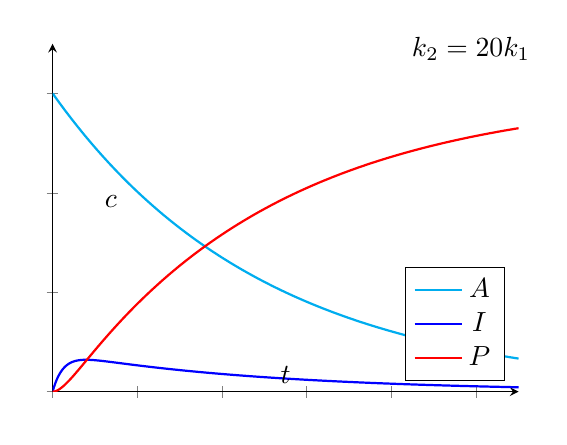
\begin{tikzpicture}
    \begin{axis}[
        title = {$k_2=20k_1$},
        title style={at={(0.75,1)},anchor=north west},
        width = 7.5cm,
        height = 6cm,
        legend pos = south east,
        x label style={at={(axis description cs:0.5,0.1)},anchor=north},
        y label style={at={(axis description cs:0.125,0.5)},rotate=270,anchor=south},
        xlabel = {$t$},
        ylabel = {$c$},
        axis lines = left,
        ymax = 3.5,
        domain = 0:5.5,
        samples = 400,
        xticklabels={},
        yticklabels={}
    ]
    \addplot [thick, cyan] {3*e^(-0.4*x)};
    \addplot [thick, blue] {3/7.6*(e^(-0.4*x)-e^(-8*x))};
    \addplot [thick, red] {3*(1+(0.4*e^(-8*x)-8*e^(-0.4*x))/7.6)};
    \legend {$\con{A}$,$\con{I}$,$\con{P}$}
    \end{axis}
\end{tikzpicture}
\end{document}